\documentclass[mathsans]{beamer} % スライド用のレイアウト
\usepackage{luatexja} % Beamer単体では日本語を出力できないのでこれを使う


\renewcommand{\kanjifamilydefault}{\gtdefault} % 漢字をゴシック体に指定
\renewcommand{\figurename}{図}
\renewcommand{\tablename}{表}
\setbeamertemplate{caption}[numbered]
\usetheme{metropolis} % usepackageじゃなくてusethemeだから注意
\usefonttheme{professionalfonts}

\usepackage{mathtools} % amsmath の拡張パッケージ
\usepackage{siunitx} % 単位に関するパッケージ
\usepackage{physics} % 物理量に関するパッケージ
\usepackage{thm-restate}

\RenewCommandCopy{\qty}{\SI}

% siunitx で数式を扱う
\newcommand{\SIeq}[2]{\SI[parse-numbers=false, per-mode=symbol]{#1}{#2}}
\newcommand{\sis}[1]{\si[per-mode=symbol]{#1}}
\newcommand{\SIs}[2]{\SI[per-mode=symbol]{#1}{#2}}


% \sisetup{
%   detect-all = false,
%   unit-font-command = \text{\rmfamily}
% }

\title{フィードバック付きDCDCコンバータ}
\author{5班 市川弦慈}
\date{\today}

\begin{document}
\begin{frame}
	\maketitle
\end{frame}
\begin{frame}
	\frametitle{実験の概要}

	\begin{enumerate}[実験\arabic*.]
		\item 加算器+比較器(図\ref{fig:add_comp})
		\item フィードバック付きDCDCコンバータ(図\ref{fig:DCDC_add_comp})
	\end{enumerate}
	$R_0=\SIs{10}{\kilo\ohm},V_\mathrm{ref}=\SIs{8.03}{\volt}$ \\
	三角波 : $\SIs{100}{\kilo\hertz}, \SIs{13}{\volt}\text{(peak-to-peak)}\eqcolon V_\mathrm{pp}$\\
	$V_+=\SIs{15}{\volt},V_-=\SIs{15}{\volt}$
	\begin{columns}
		\begin{column}{.45\linewidth}
			\begin{figure}[htbp]
				\begin{center}
					\scalebox{0.08}{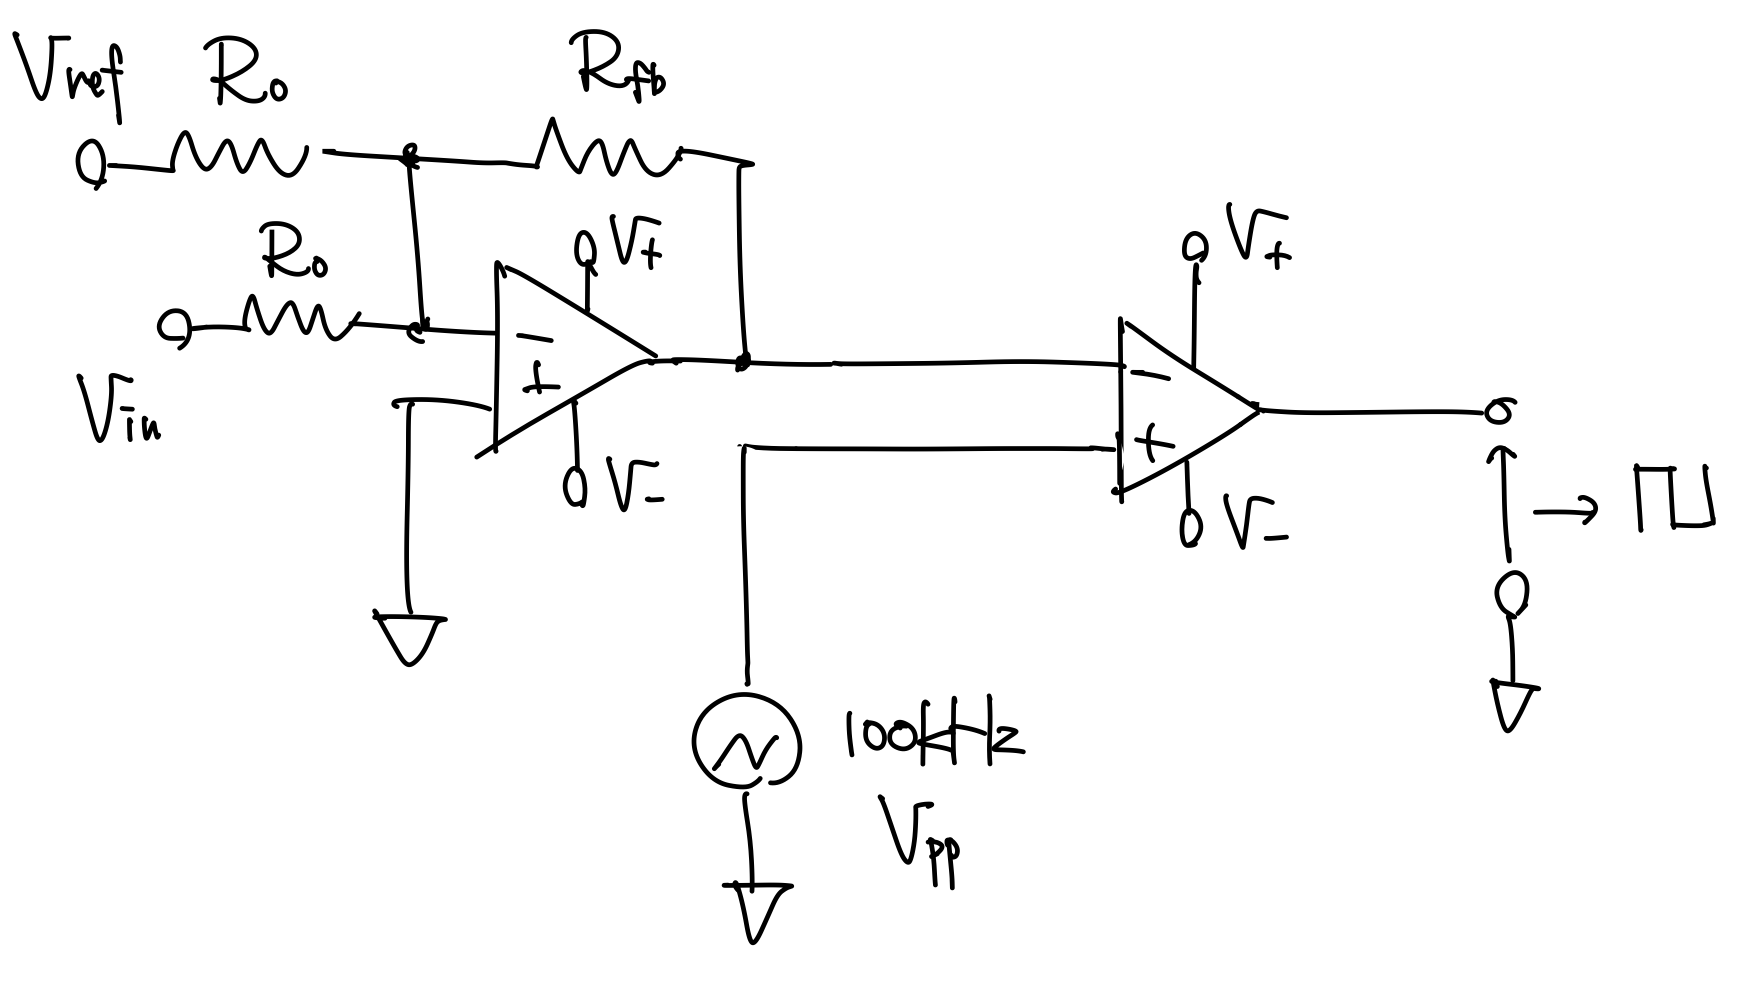
\includegraphics{../figures/3_1.png}}
					\caption{実験1の回路図}\label{fig:add_comp}
				\end{center}
			\end{figure}
		\end{column}
		\begin{column}{.45\linewidth}
			\begin{figure}[htbp]
				\begin{center}
					\scalebox{0.08}{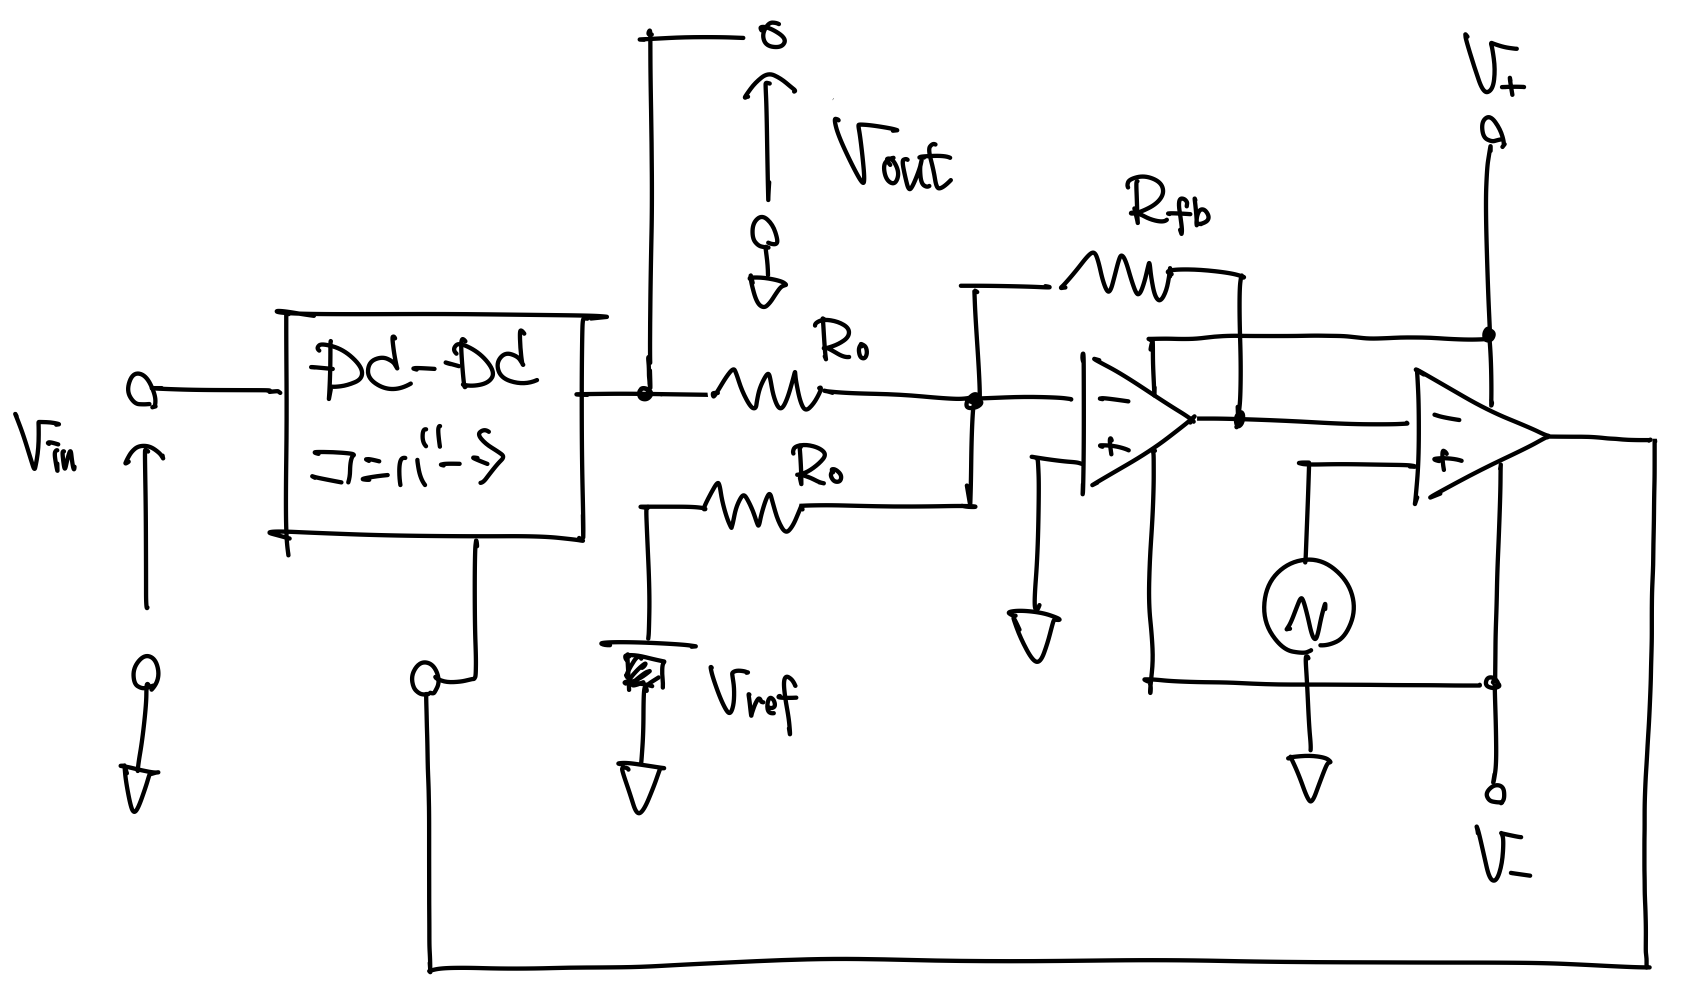
\includegraphics{../figures/3_2.png}}
					\caption{実験2の回路図}\label{fig:DCDC_add_comp}
				\end{center}
			\end{figure}
		\end{column}
	\end{columns}
\end{frame}
\begin{frame}
	\frametitle{実験の概要(実験1)}
	比較器から出力される方形波のデューティ比の理論値$D_\mathrm{thm}$
	\begin{align}
		K_\mathrm{fb}  & = -\frac{R_\mathrm{fb}}{R_0}                                                        \\
		D_\mathrm{thm} & = \frac{1}{2} - \frac{K_\mathrm{fb}}{V_\mathrm{pp}}(V_\mathrm{ref}-|V_\mathrm{in}|)
	\end{align}
	\hrulefill\\
	DCDCコンバータの入出力電圧$V_\mathrm{in},V_\mathrm{out}$の関係
	\begin{align}
		V_\mathrm{in} = - V_\mathrm{out} \cdot\frac{V_\mathrm{pp}-2K_\mathrm{fb}(V_\mathrm{ref}+V_\mathrm{out})}{V_\mathrm{pp}+2K_\mathrm{fb}(V_\mathrm{ref}+V_\mathrm{out})}
	\end{align}
\end{frame}
\begin{frame}
	\frametitle{結果}
	\begin{enumerate}[実験\arabic*.]
		\item それぞれの測定点について理論値よりも大きいデューティ比になった.
		\item 理論線に沿った点群が見られたが,入力電圧が大きいところでは誤差が大きいように見られた.
	\end{enumerate}
	\begin{columns}
		\begin{column}{.5\linewidth}
			\begin{figure}[htbp]
				\begin{center}
					\scalebox{0.35}{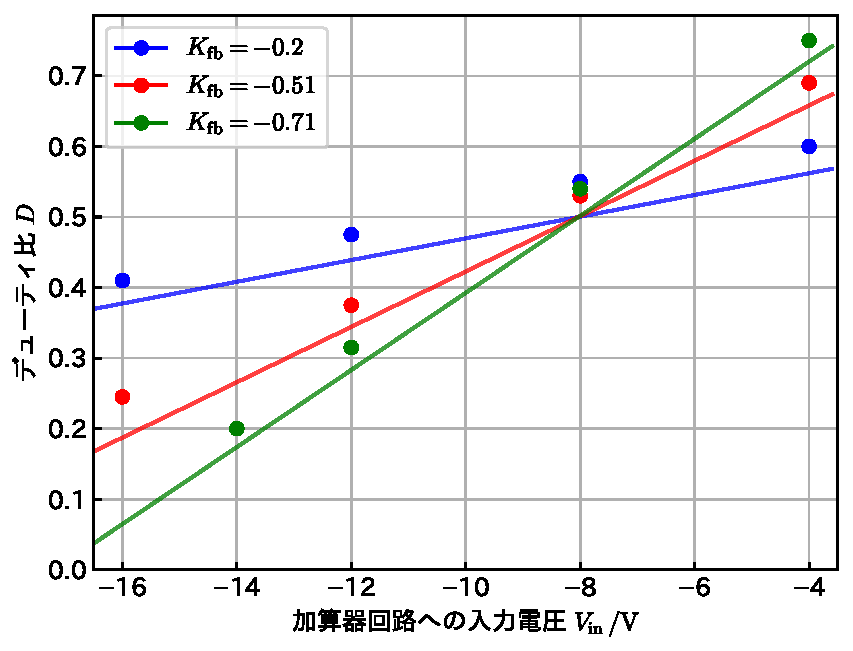
\includegraphics{../figures/3_add_comp.pdf}}
					\caption{実験1の結果}\label{fig:exp_add_comp}
				\end{center}
			\end{figure}
		\end{column}
		\begin{column}{.5\linewidth}
			\begin{figure}
				\begin{center}
					\scalebox{0.35}{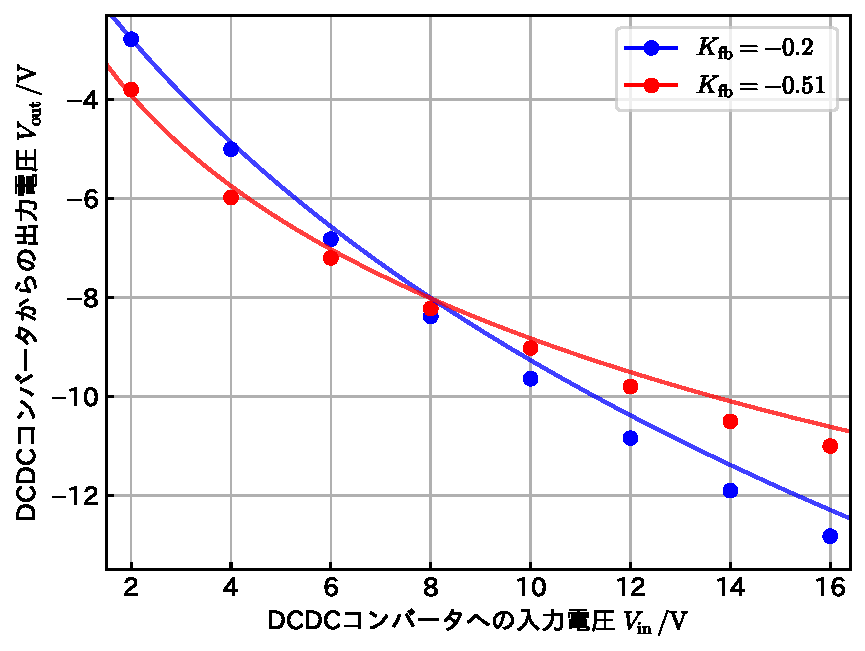
\includegraphics{../figures/3_DCDC_add_comp.pdf}}
					\caption{実験2の結果}\label{fig:exp_DCDC_add_comp}
				\end{center}
			\end{figure}
		\end{column}
	\end{columns}
\end{frame}
\begin{frame}
	\frametitle{考察(実験1)}
	\begin{columns}
		\begin{column}{.45\linewidth}
			\begin{itemize}
				\item 比較器のスルーレートにより理想的な方形波が出力されなかった.
				\item 方形波のオン時間の定義(実験中に定義)が適切でなかった.
			\end{itemize}
			ことがずれの原因
		\end{column}
		\begin{column}{.5\linewidth}
			\begin{figure}[htbp]
				\begin{center}
					\scalebox{0.35}{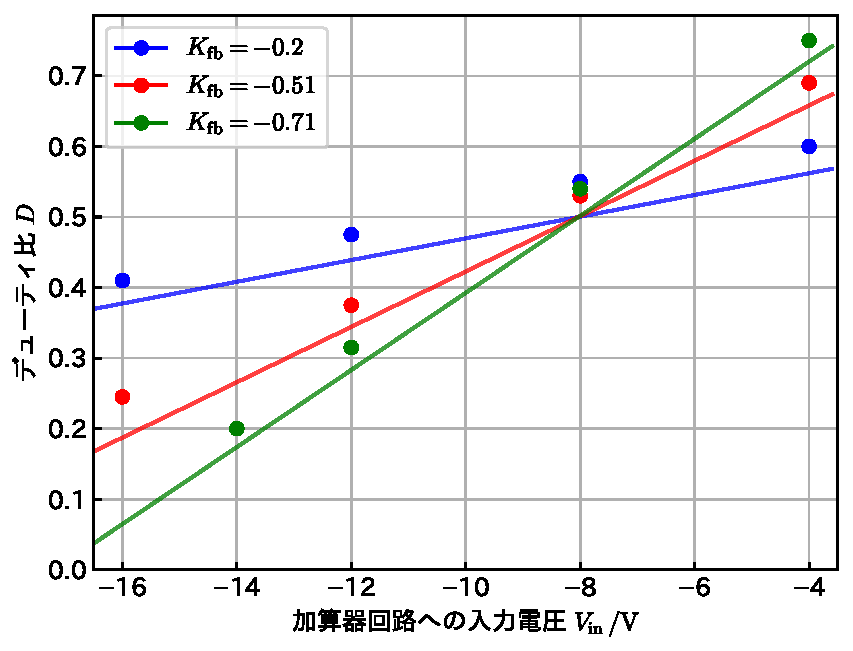
\includegraphics{../figures/3_add_comp.pdf}}
					\vspace{-1em}
					\caption*{図 \ref{fig:exp_add_comp}(再掲) : 実験1の結果}
				\end{center}
			\end{figure}
		\end{column}
	\end{columns}
\end{frame}
\begin{frame}
	\frametitle{考察(実験2)}
	\begin{columns}
		\begin{column}{.45\linewidth}
			\begin{itemize}
				\item デューティ比が小さく,スルーレートの影響が顕著になる
			\end{itemize}
			ことがずれの原因
		\end{column}
		\begin{column}{.5\linewidth}
			\begin{figure}[htbp]
				\begin{center}
					\scalebox{0.35}{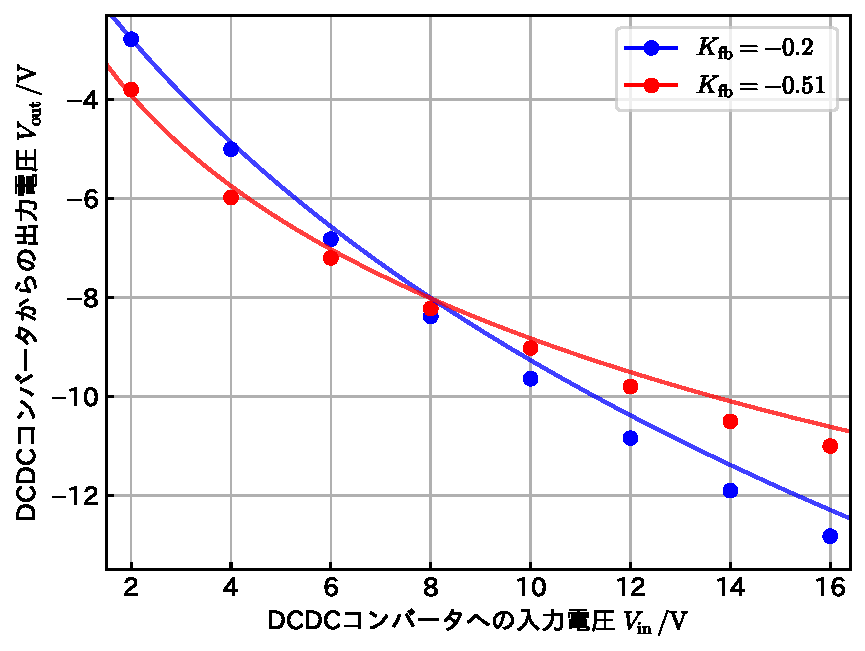
\includegraphics{../figures/3_DCDC_add_comp.pdf}}
					\vspace{-1em}
					\caption*{図 \ref{fig:exp_DCDC_add_comp}(再掲) : 実験2の結果}
				\end{center}
			\end{figure}
		\end{column}
	\end{columns}
\end{frame}
\end{document}